\documentclass[12pt]{article}
\usepackage{graphicx} % Required for inserting images
\usepackage[margin = 1in]{geometry}
\usepackage{amsmath}
\usepackage{amsthm}
\usepackage{amssymb}
\usepackage{todonotes}
\usepackage{booktabs}

%\RequirePackage[backend=biber,sorting=nty, style=chicago-authordate, natbib=true, hyperref=true, backref=false, isbn=false]{biblatex}  % reference manager
%\DeclareLanguageMapping{american}{american-apa} %added

\usepackage[authordate,backend=biber,ibidtracker=false,uniquename=false,maxcitenames=3,dashed=false]{biblatex-chicago}



\renewcommand{\footnoterule}{%
  \kern -3pt
  \hrule width \linewidth height 0.5pt
  \kern 2.6pt
}

\usepackage{setspace}
\usepackage{chngcntr}
\usepackage{hyperref}
\usepackage{longtable}
\usepackage{float}




\setlength{\tabcolsep}{4pt}

%\RequirePackage[backend=biber,sorting=nty, style=chicago-authordate, natbib=true, hyperref=true, backref=false, issn=false, isbn=false]{biblatex}

\doublespacing
\addbibresource{bib/PoliceResidency.bib}

\title{Estimator Selection Diagnostics in Staggered Differences-in-Differences}
\author{Eric Dobbie}
\date{\today}

\begin{document}

\maketitle

\begin{abstract}
    \noindent In settings with staggered treatment adoption, two-way fixed effects estimators have been shown to produce biased estimates of the average treatment effect on the treated (ATT) when treatment effects are heterogeneous. A family of estimators addresses this problem through reweighting of ``clean comparisons,'' where the bias inducing comparisons to earlier treated units are removed from the analysis. I demonstrate this weighting phenomenon through an application to \textcite{payson2025residency}, which studies the effect of police residency requirements on fatal encounters, a policy setting with staggered adoption across municipalities. I show that the weights given to individual clean comparisons are determined exclusively by panel geometry and that these weights do not necessarily correspond in favorable ways to the ability to assess parallel trend violations within each comparison. Researchers can recover all possible weighting vectors ex-ante, without specifying an outcome model, and see if they are able to identify meaningful pre-trends with outcome variance.
\end{abstract}
% Add to abstract: imputation estimators

\newpage

\section{Introduction}

%Target word count: 900

Differences-in-Differences (DiD) is a commonly used method in political science. In order to estimate causal effects of policy interventions, DiD approaches compare units that have received the policy change to those that have not received the policy change under the assumption that the outcome of interest would have changed the same way in each unit absent the intervention. According to \textcite{chiu2026causal}, two-way fixed effect (TWFE) models are the predominant method for analyzing panel data for causal identification, with 64 out of 102 studies published in leading political science journals utilizing a TWFE model for their analysis. In applied political science work, policy treatments are often staggered as different geographical areas apply the policies at different times. If the timing of these treatments changes the effect of the treatment, then the TWFE estimators that are commonly applied in these settings will be biased. 

The econometrics literature on correcting this bias has been extraordinarily active over the last several years \parencite{callaway2021difference, sun2021estimating, borusyak2024revisiting, gardner2022two, goodman2021difference,baker2022much, baker2026difference}. While a wide variety of solutions have been proposed and guidelines for estimator selection do exist, there is little actionable advice on diagnostic tests that can be conducted without introducing multiple testing concerns. Among the current guidance, \textcite{chiu2026causal} suggest using imputation estimators because they have more power (from using all pre-treatment periods) and match closer to TWFE in the outcome model. \textcite{roth2023s} point out that researchers face an efficiency-robustness tradeoff in estimator selection based on parallel trends assumptions, which serves as a basis for estimator selection. \textcite{callaway2023difference} makes this view more concrete by pointing out that the differences in parallel trends assumptions can be boiled down to the following comparison: More periods involved in the pre-trend leads to more efficient estimation; fewer periods, such as a universal base period, leads estimates being more robust to violations in some periods of the panel.

This paper contributes to this literature by showing that while both the aggregation weights (that take clean comparisons and combine them into event study, cohort, calendar, or a single ATT effects) and the ability of researchers to detect pre-trend violations within the clean comparisons are a direct function of panel geometry and the outcome alone (treatment timing, cohort size, outcome variance). Crucially, there is no guarantee that highly weighted comparisons will be those that are ``checkable''\footnote{Checkable, or ``checkability'', in this context, means able to detect a reasonably sized PT violation.}. As the aggregation weights for each class of estimator are able to be diagnosed without an outcome model, researchers can evaluate their estimator selection by observing weights against checkability and utilizing the estimator that gives the most purchase on PT. 

To demonstrate this property I will utilize an application of \textcite{payson2025residency} present an analysis of police residency requirements. Residency requirements, as the name suggests, are a policy intervention whereby municipal employees are required to live in the municipality in which they work\footnote{Alternate definitions of residency requirements often include rules that dictate municipal employees must live within a predetermined distance of the city rather than strictly inside city limits. However, for this paper, the strict definition will be used throughout for consistency with the choices of \textcite{payson2025residency}.}. The logic behind residency requirements is that officers who interact with members of a community will be less likely to discriminate against them, and requiring officers to live in the community leads to forced contact with the discriminated against group, which could give them a sense of empathy for those in the community \parencite{hopkins_politicized_2010, pettigrew_recent_2011, hubert_social_2022}. The authors estimate the effect of removing a residency requirement on two outcomes: the racial composition of the force and the probability of a fatal police-civilian encounter in an agency-year. I focus on the latter. 

The primary specification of \textcite{payson2025residency} is TWFE, and they engage the staggered-timing literature through a stacked design with clean controls, entropy balancing, and cohort-exclusion checks \parencite{cengiz2019effect}. They find that removing a residency requirement reduces the probability of a fatal encounter by roughly 9 to 10 percentage points, against a base rate near 31 percent. This approach meets any reasonable standard set for applied researchers in the staggered treatment literature. However, the panel structure of their data makes it an illustrative case for the ways researchers can use ex-ante checks of aggregation weights and checkability to inform estimator selection.

%needed for intro, add imputation estimators and modify the contribution paragraph

%Next part is goodman bacon bias and reweighting estimators

\section{Staggered Treatments Lead to Bad Comparisons}

%Target word count: 900

The problem with the classic TWFE approach is so-called ``forbidden comparisons'' where treated units act as controls for units treated in later time periods. While the estimate produced by the TWFE estimator can be decomposed into all possible $2\times2$ DiD estimates \parencite{goodman2021difference}, this decomposition does not require the weights on each individual $2\times 2$ DiD estimate to be positive. The negative weights can lead to problems where every treatment cohort has an effect of one sign and the TWFE estimator gives the opposite sign. While current evidence suggests that the sign flipping problem is rare in applied settings \parencite{chiu2026causal}, the comparisons that cause these problems are still relatively counter-intuitive and lead to difficulty in interpreting the results of the analysis.

Fundamentally, the solution to the problem is intuitive; researchers must restrict their analysis down to the clean comparisons and then recombine them through aggregation. By ``clean comparisons,'' I mean the comparisons to never-treated or not-yet-treated units. These are the exact comparisons that remain uncontaminated by the bias outlined in \cite{goodman2021difference} when treatment effects vary across time within treatment cohorts. 

In this paper, I will use the application to \cite{payson2025residency} to establish this panel geometry quality for these estimators that estimate $2 \times 2$ comparisons directly using clean comparisons and then aggregate them together, which I will refer to as reweighting estimators. Explicitly, I will utilize \textcite{sun2021estimating}, \textcite{callaway2021difference}, and stacked regression \parencite{baker2022much, cengiz2019effect, wing2024stacked} as direct reweighting estimators. Additionally, I will show that these same properties hold for imputation estimators \parencite{gardner2022two, borusyak2024revisiting}. Stacked regression is the selected estimator used as a robustness check in \textcite{payson2025residency}. Each estimator can be directly traced back to effects estimated for a cohort in each post-treatment time period. Through this replication process, I will demonstrate that under treatment effect heterogeneity these estimators can produce competing results, as they allow for different comparisons and weight the resulting estimates for aggregation differently. I will then discuss the ways applied researchers should adjudicate between potentially competing result sets.

To establish notation that will be used throughout the remainder of the paper, treatment cohorts are indexed by their treatment timing $g$. For example, a cohort that is treated in $2000$ will be represented as the $g = 2000$ treatment cohort. Time, irrespective of treatment timing, will be represented by the index $t$. This could also be referred to as calendar time. Event time, represented by index $e$, refers to the distance from treatment. As an example, in $t = 2001$, for $g = 2000$, event time is $e = 2001 - 2000 = 1$, and for $g = 2005$, the same calendar time gives $e = 2001 - 2005 = -4$. 


\subsection{How Clean Comparisons are Constructed}\label{sec:cc_const}

Each of these reweighting estimators has a common target, a clean $2 \times 2$ comparison to a selected control group. Within each estimator, there are some researcher degrees of freedom in the construction of these sets, and they vary by estimator. The primary choice to be made is whether the comparison group will be comprised of never-treated or not-yet-treated observations\footnote{The package defaults for each of these estimators is to use never-treated units as controls.}.

In order to build out a stacked regression, the researcher first constructs a separate dataset, or  ``stack,'' for each adoption cohort $g$.\footnote{For a more detailed overview of building out a stacked dataset, see \textcite{wing2024stacked}.} Each stack is restricted to an event ``window'' around $g$, such that $k_p$ periods before and $k_a$ periods after treatment are included in the stack. These stacks contain never-treated controls, or, at researcher discretion, can contain not-yet-treated units that never enter treatment through period $g+k_a$. These controls can be shared across stacks such that the same control unit appears across many (or all) stacks. This leads to a sub-experiment within each stack such that treatment timing does not vary within the stack. A pooled effect is then directly estimated using the following model:


\begin{equation}\label{eq:interactive}
    Y_{igt} = \beta_1 D_{igt} + \lambda \mathbf{X}_{it} + \gamma_{ig} + \delta_{tg} + \epsilon_{igt}
\end{equation}

Where $\beta$ is the pooled treatment effect, $\mathbf{X}_{it}$ is a vector of covariates, $\gamma$ is a unit-by-stack fixed effect, $\delta$ is a time-by-stack interacted fixed effect, and $\epsilon$ is the error term.

\subsection{How Clean Comparisons are Aggregated}\label{sec:aggregation}

While \textcite{callaway2021difference} propose using the $ATT(g,t)$ as the target estimand of staggered treatment DiD, in settings with many adoption cohorts and/or time periods interpreting these individual comparisons might not be directly possible. Generally, there are four primary aggregation targets that are easily characterized for each of these reweighting estimators: (1) calendar effects, (2) event study effects, (3) cohort level effects, and (4) a single ATT. Calendar effects are targeting the effect in each time period $t$, irrespective of the treatment timing.

As described above, stacked regression is typically estimated as a single pooled regression with one ATT as the target. Despite this, it still fits in the class of reweighting estimators as the comparisons within each stack are always clean and the pooled effect is a non-negatively weighted average of stack-specific effects (see Appendix). \textcite{wing2024stacked} show this convex decomposition when the treatment share is constant across stacks. However, the result presented in the appendix generalizes their finding to any stacked panel regardless of treatment share or panel balance. Fundamentally, stacked regressions targets a single pooled ATT with the same building blocks, the $\text{ATT}(g,t)$, under an implicit weighting scheme. \textcite{wing2024stacked} and the generalized proof in the appendix show that these weights are given by the share of residualized treatment variation within the stack-specific effects.\footnote{It is also possible to form calendar effects and event study estimates using a stacked regression framework, as shown in \textcite{cengiz2019effect} and \textcite{wing2024stacked}. For the purposes of this replication, the focus is limited to disaggregation to cohort-level effects.}

\section{Aggregation Weights and Checkability are Functions of Panel Geometry}

For the following sections I will focus on aggregation to a single ATT\footnote{I do this for a variety of reasons. First, many applied researchers are aiming to report a single ATT in their analysis, and it is a common target estimand in staggered DiD designs. Second, It is the only target that all of these estimators report in their standard implementation, making it the best estimand for comparing across estimators. The mismatch between weight and
checkability is not specific to this target, but its severity varies with the aggregation, as Section~\ref{sec:diverge} discusses.}. All of these modern estimators discussed above report, either explicitly or implicitly, a weighted average of cohort-time effects:
\begin{equation}\label{eq:theta}
    \theta = \sum_g \sum_{t\geq g} w_{g,t} \tau_{g,t}
\end{equation}

where weights are greater than or equal to zero and sum to one.

\subsection{Weights}            % Prop 1 -> appendix; CS/imputation menus

The weights in this aggregation are a function of what I will refer to as panel geometry. By panel geometry, I mean adoption times, cohort sizes, and the window over which outcomes are observed in the panel. Importantly, panel geometry is fixed for any selected dataset and outcome prior to running any models of the outcome, so the weights can be inspected prior to running any analysis.

For \textcite{callaway2021difference} and the imputation estimators \parencite{borusyak2024revisiting}, weights are selected from a set of possible weighting vectors. The simple aggregation weights every estimable post-treatment cell by it's cohort size, so a cohort's total weight is 

\begin{equation}\label{eq:cs_simple}
    W_g = \frac{n_g \cdot \text{post}_g}{\sum_{g'} n_{g'} \cdot \text{post}_{g'}}
\end{equation}

where $n_g$ is the cohort size, $\text{post}_g$ is the number of periods observed after treatment.

Event-study aggregation weights cohorts by their share among those observed at each time $e$. \textcite{sun2021estimating} uses these same shares. Imputation estimators aggregate imputed effects with either of these options, with defaults to Equation \ref{eq:cs_simple}.

Stacked regression does not allow for explicit weight selection. Instead, its pooled coefficient is a weighted average of stack-specific coefficients with $w_s = V_s / V$, the stack's share of residualized treatment variation.\footnote{See Proposition 1 of the proof in the appendix} For a balanced stack without covariates:

\begin{equation}\label{eq:stacked_weights}
    V_s = N_s T_s p_s(1-p_s)q_s(1-q_s)
\end{equation}

where $p_s$ is the share of the stack's units that are treated and $q_s$ is the share of its periods that are post-treatment. Within a stack, $\hat{\beta}_s$ weights the cohort's post-treatment periods equally.

Computing these expressions requires no modeling of the outcome. Every estimator's weights can be computed and compared before any model is run. What these weights cannot reveal is whether the cohorts they favor are the ones whose identifying assumptions can be checked.

\subsection{Checkability}       % three inputs; footnote definition

A cohort's parallel trends assumption is \emph{checkable} if a pre-trend test exists against the comparison group used to estimate it's effect and \emph{well checked} if that test can detect a violation of substantively meaningful size. Whether a test exists depends on three features of panel geometry.

The first is the number of pre-treatment periods in the data, $\text{pre}_g = g - t_0$, where $t_0$ is the first period with observed outcomes. With one pre-treatment period there is no trend to test. With two pre-treatment period the test reduces to a single year-to-year contrast, which can be identified. I treat cohorts with fewer than two pre-treatment periods as uncheckable.

The second is a comparison group that remains untreated throughout the pre-treatment window and is the same group used in estimation. When the comparison group is fixed, such as the never-treated controls in \textcite{callaway2021difference} and \textcite{sun2021estimating} or each stack's clean controls in stacked regression, using an event study from the pre-treatment periods satisfy this condition by construction. When the comparison group is not fixed, the condition only sometimes holds. Estimators that use not-yet-treated units, as is a package option in \textcite{callaway2021difference} and used by imputation estimators, each cohort is compared to a group that shrinks over time, so a pre-test against the initial comparison group matches the estimation in the first treated period \parencite{liu2025cohort}. I take $\mathcal{C}^k_g$ to be this initial group, which makes the checkability measure presented here a best-case scenario for these estimators.  

The third is the number of treated clusters. With a single treated cluster, cluster-robust and wild bootstrap tests are invalid \parencite{mackinnon2018wild}, and randomization inference requires the errors of the treated units to be exchangable with those of the control units \parencite{conley2011inference}, an assumption that the application violates.

Moving to a formal definition of checkability, let $\hat{\delta}^k_g$ be cohort $g$'s estimated linear pre-trend against $\mathcal{C}^k_g$, the comparison group estimator $k$ assignes it, and define the minimum detectable trend as

\begin{equation}\label{eq:mde}
    \text{MDE}^k_g = \begin{cases}
        (z_{1-\alpha/2}+z_{1-\kappa})\, \widehat{\text{SE}}(\hat{\delta}^k_g) & \text{if } \text{pre}_g \geq 2, \ \mathcal{C}^k_g \neq \emptyset,\ n_g \geq 2, \\
        \infty & \text{otherwise}
    \end{cases}
\end{equation}

with the standard error computed by a method valid for few treated clusters. The MDE summarizes both components of checkability: it is infinite when no valid test exists, and otherwise smaller the better the cohort is able to be checked for pre-trend violations. A cohort can be considered ``well checked'' in this framework at a researcher set tolerance $\bar{\delta}$ if $\text{MDE}_g^k \leq \bar{\delta}$, where $\bar{\delta}$ is the largest pre-trend violation the researcher would regard as harmless.\footnote{A natural benchmark is the slope whose accumulated bias would match the smallest substantive effect of interest. Under a $g-1$ baseline (as is the case in \textcite{callaway2021difference}), a linear violation of slope $\delta$ biases a cohort's average effect by $\delta (\text{post}_g + 1)/2$, so cohorts with long post-treatment windows tolerate only small pre-trends. Estimators with a pre-period-average baseline accumulate more bias from that same slope.} The diagnostic is the share of aggregation weight on cohorts that are not well checked:

\begin{equation}\label{eq:unchecked}
    U^k(\bar{\delta}) = \sum_g W^k_g \, \mathbf{1}\{\text{MDE}^k_g > \bar{\delta}\}
\end{equation}

which only depends on the outcome through pre-treatment variation. Note that $U^k(\infty)$ serves as a lower bound on unchecked weight at any finite tolerance, as it is the weight on cohorts with no valid test for pre-trends.

\subsection{Why They Diverge}\label{sec:diverge}   % pre+post=T; event-time composition; stacked V_s; windows

Both checkability and the aggregation weights derive directly from panel geometry. However, the ways in which they respond to panel geometry do not coincide, such that cohorts with high weights are not necessarily well-checked and vice-versa. While weights and checkability are both increasing in cohort size, the number of pre-treatment periods increases checkability while decreasing the weights under the weights given in Equation~\ref{eq:cs_simple}.

Substituting $\text{post}_g = T -\text{pre}_g + 1$ into Equation~\ref{eq:cs_simple}:

\begin{equation}\label{eq:diverge}
    W_g \propto n_g \, (T - \text{pre}_g + 1),
\end{equation}

so, holding cohort size fixed, each additional pre-treatment period lowers a cohort's weight under the simple aggregation. The same additional periods lower the minimum detectable pre-trend with $[\text{pre}_g(\text{pre}_g^2 - 1 /12)]^{1/2}$. Early adopters are, as a consequence of this, weighted higher with lower checkability. They are also the cohorts that, under a $g-1$ baseline, can only sustain a small pre-trend before the bias accumulates over many post-treatment periods to match reasonable effect sizes. This means that the least checkable cohorts also have the lowest tolerance for violations.

The severity of this issue depends on the aggregation scheme. Event-study effects over long time-horizons are identified only by the early adopting cohorts \parencite{liu2025cohort}, so they depend on the lease checkable cohorts in the panel. Cohort-level aggregation depends only on the relative size of the cohort, removing $\text{post}_g$ from Equation~\ref{eq:cs_simple} and, along with it, the link between weights and checkability.

Stacked regression's weights depend on how the stacks are built by the researcher. Under the full panel stacked construction used by \textcite{payson2025residency}, where all observed periods are used for each cohort, the weights follow from the share of periods within the stack that are post-treatment, $q_s(1-q_s)$. This means that weights are highest for mid-cohort adopters. Whether or not these mid-panel cohorts are checkable depends on the numebr of pre-treatment periods. The windowed construction of \textcite{cengiz2019effect} behaves differently. When every stack spans the same $k_p$ pre-treatment and $k_a$ post-treatment periods, $T_s$ and $q_s$ are common across stacks and Equation~\ref{eq:stacked_weights} reduces to
\begin{equation}\label{eq:stacked_window}
    w_s \propto \left(\frac{1}{n_g} + \frac{1}{n_c}\right)^{-1}
\end{equation}
where $n_c$ si the number of clean controls in the stack. Because every stack also has the same number of pre-treatment periods, the minimum detectable trend under independent errors is proportional to $(1/n_g + 1/n_c)^{1/2}$, meaning that windowed stacked regression weights cohorts in proportion to the precision of the stack's pre-trend test, $w_s \propto \text{MDE}_g^{-2}$. The alignment of weights with checkability is a strength of the windowed stacked regression. However, it is important to acknowledge that this alignment comes with costs. Cohorts with fewer than $k_p$ pre-treatment periods or $k_a$ post-treatment periods are dropped, which changes the estimand. The alignment is also relative rather than absolute, the most well-checked cohorts might not actually be checkable under a given window. Additionally, stacks with one treated cluster will receive weight with no valid test for checkability, so the alignment does not hold in that case.




\subsection{Tests Inherit the Geometry} % Liu Lemma 1 at e=0; CSX Hausman power

% This is the core of the unwritten parts of the paper. Pulling down the FWL part helps to establish this for stacked, demonstration of it for CS and imputation follows from there
%Word count budget: 1,400 words (it might be more)

\section{Application to \textcite{payson2025residency}}

%the core application of the argument: what does the ex-ante geometry test show us and what happens if we just ran each estimator? When would we have reported results based on uncheckable comparisons?
%Target: 1,800 words (it's going to be more, probably)

\textcite{payson2025residency} first estimate a TWFE model to identify the ATT of removal of a residency requirement on the probability of a fatal encounter, finding a reduction in probability of $~9\%$. As a first diagnostic step, this finding can be decomposed according to \textcite{goodman2021difference} decomposition to see whether contaminated comparisons are entering the estimated effect.

The econometric specification used to estimate the stacked regression presented in \textcite{payson2025residency} is:

\begin{equation}\label{eq:add_model}
    Y_{igt} = \beta D_{igt} + \lambda \mathbf{X}_{it} + \gamma_{i} + \delta_{tg} + \epsilon_{igt}
\end{equation}

Where, similar to the model in Equation \ref{eq:interactive}, $\beta$ is the pooled treatment effect, $\mathbf{X}_{it}$ is a vector of covariates,\footnote{Specifically, log scaled city population, log scaled median income in the city, the percent of the city population that is white, and percentage of officers that are white. City level covariates are drawn from the 2005-2020 American Community Survey. Prior to 2005, the city level covariates are interpolated from decennial Census results. Officer demographics are drawn from LEMAS surveys that are conducted periodically with 9 surveys fielded from 1987 to 2020. The annual counts are imputed from these surveys.} $\gamma$ is a unit (city) level fixed effect, $\delta$ is a time-by-stack interacted fixed effect, and $\epsilon$ is the error term. This specification is what the replication code actually estimates, but careful readers will notice that $\gamma$ is not estimated as a unit-by-stack effect. This does not appear to be an intentional decision by the authors, as their econometric specification described in their paper includes an agency-by-stack fixed effect. 


Table \ref{tab:spec-grid} shows that the additive specification reproduces the reported results in Table 5 of \textcite{payson2025residency}. Correcting this coding error does not substantively alter the pooled point estimate. However, as the proof in the appendix demonstrates (see Lemma 1, in particular), a stack-interacted fixed effect is mathematically required to decompose the pooled ATT into valid stack-specific estimates. Because control agencies are repeated across sub-experiments, an additive unit fixed effect forces them into a single global baseline. This generates structural dependence across the first-order conditions and causes cohort-level estimates to herd together, effectively masking underlying treatment effect heterogeneity across stacks. The corrected specification, featuring interacted agency-by-stack fixed effects, is defined in Equation \ref{eq:interactive} above. Unless noted otherwise, minor discrepancies with the published estimates in \textcite{payson2025residency} stem directly from this correction.


\subsection{Stack Construction}

The full panel of data used for the base TWFE specification has 15 treatment cohorts.\footnote{A full description of the data is available in Table \ref{tab:data-description}.} For each treatment cohort, they construct a stack using all non-changers over the panel, such that the comparison is made up of never-treated and always-treated units. Table \ref{tab:stack-composition} shows the full composition of each stack with the number of cites that drop a requirement, adopt a requirement, the number of never-treated controls, and the number of always-treated controls. 

In general, the use of never-changing units as controls rather than never-treated units might be ill-advised. Always-treated units, in most policy settings, entered treatment at some unobserved point in time before the beginning of the panel. If treatment effects change over time then \textcite{goodman2021difference} shows that these are the exact forbidden comparisons that lead to bias in TWFE. In this setting, treatment adoption means the removal of a policy, which is a strange ``always-treated'' state to be in, it could mean that a city had a policy at some point before the panel begins or that they never had a policy at all. For this to lead to bias in the estimated effects in the stacked specification, one would need to believe that the treatment effect of not having a policy was changing \textit{within the panel} for units treated before the panel. In this specific setting, units are observed if their treatment status changes from 1987 to 2000 before the fatal encounters data begins and excluded from the analysis if they enter or leave treatment in that time period. As a result, bias only comes from treatment dynamics over 13 years post treatment. If the analysis is redone with only never-treated controls, the results do not meaningfully change, which makes sense based on how far downstream treatment dynamics would need to be for results to change based on the inclusion of these always-treated controls.


In constructing a stacked dataset, researchers must make choices about the number of periods to include before and after treatment within each stack. \textcite{payson2025residency} utilize the full panel of available data in the construction of the stacked datasets, which is in contrast to standard stacked dataset construction \parencite{cengiz2019effect, baker2022much, wing2024stacked} where a standard number of pre-treatment and post-treatment periods must be included for each stack. This means that there is variation introduced in the number of pre-treatment and post-treatment periods across cohorts. For example, the stack at $g = 2018$ has 18 pre-treatment periods and 3 post-treatment periods while the stack at $g = 2004$ has 4 pre-treatment periods and 17 post-treatment periods. The consequence of this is that early adopters provide more years of post-treatment data, which could skew the pooled estimate if the treatment effect is dynamic over time. Additionally, as stacks require parallel trends to hold over the full pretreatment periods, later adopters face a rather strict version of the parallel trends assumption whereby parallel trends must hold for the full pre-treatment time span.

To test sensitivity to the number of included periods, the stacks can be reconstructed using a variety of temporal bounds.\footnote{For this exercise I will utilize a symmetrical window around treatment timing such that, in the notation of Section \ref{sec:cc_const}, $k = k_p = k_a$ and each stack includes periods $[g - k, g+k]$. The symmetric window is not necessary, it simply reduces the number of possible windows.} Figure \ref{fig:window} shows how various symmetric windows change the pooled coefficient from the stacked regression. The X-axis in the figure represents the window hal-width, or the number of pre-treatment and post-treatment periods. The Y-axis tracks the pooled regression coefficient with shaded $95\%$ confidence intervals. Each point is labeled with the number of eligible cohorts for that set symmetric window size. Notice that the number of eligible cohorts reduces as the window size increases. This is a consequence of the number of years in the panel. Once the window requires too many periods for a unit to provide a full window of support, that cohort drops from the stacked dataset. 

\begin{figure}
    \centering
    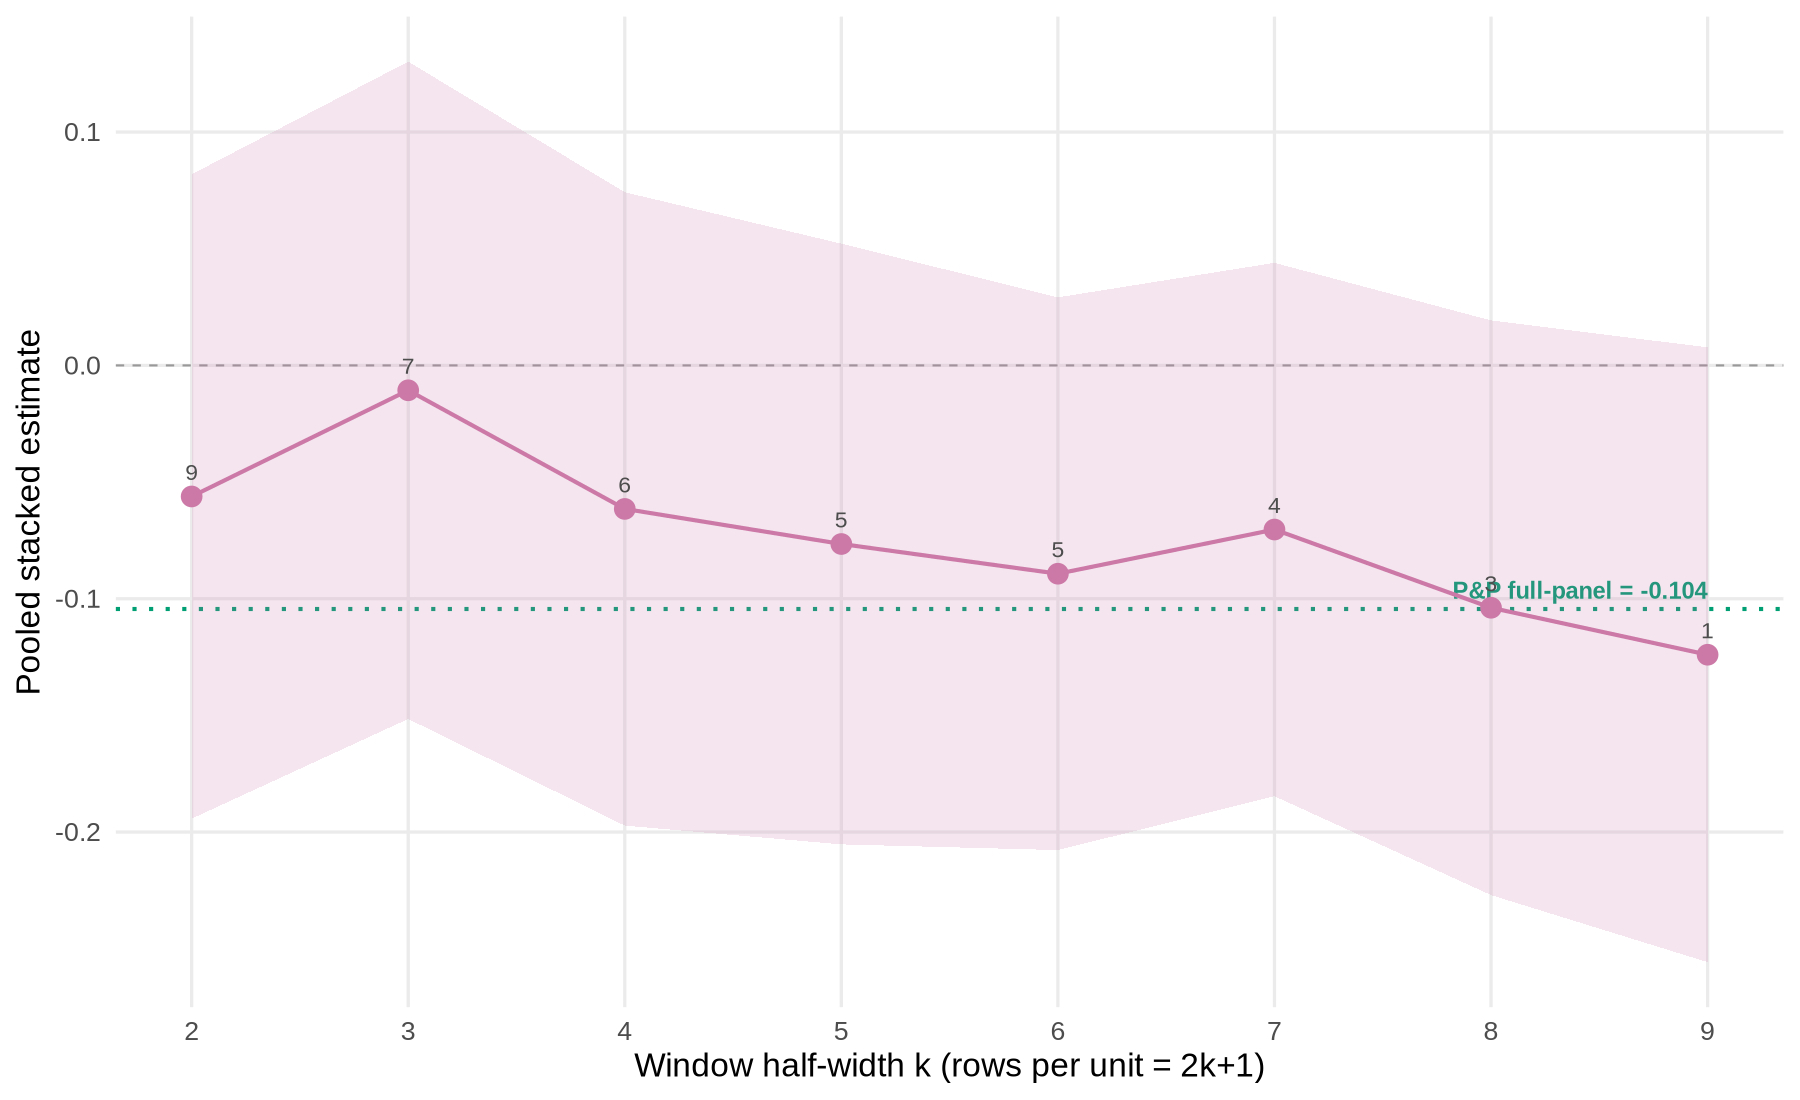
\includegraphics[width=0.75\linewidth]{figures/cengiz_window_sensitivity.png}
    \caption{Varying symmetric window around treatment timing for stack construction.}
    \label{fig:window}
\end{figure}

By varying the windows from $\pm 2$ to $\pm 9$ periods pre-and-post treatment, the sensitivity of the negative, significant result to windowing becomes clear. First, for no symmetric window is the point estimate significant at $95\%$ confidence levels. Second, the magnitude of the estimated effect is substantially reduced at smaller windows, with the narrowest windows moving close to zero effect. The effects converge towards the full sample estimated effect as the number of periods increases and more of the boundary cohorts drop from the estimation. This is partially an artifact of the 2009 cohort effect being proximate to the pooled effect in addition to it being the only cohort that fully survives the expansion of the window to $\pm 9$.


\subsection{Stack Decomposition}

As described in section \ref{sec:aggregation}, the single pooled effect reported by stacked regression can be decomposed into cohort level effects. These cohort level effects are identical to running a standard TWFE model on the stack itself. Table \ref{tab:cohort-weights} reports each stack's estimated effect ($\hat{\beta}$) and weight contributed to the pooled effect estimated using the econometric specification in Equation \ref{eq:interactive} without covariates.

\begin{table}[t]\centering
\caption{Cohort-level contributions to the pooled stacked estimate.}
\label{tab:cohort-weights}
\begin{tabular}{lrrcrr}
\toprule
Stack & Treated & Controls & Identified & $w_s$ & $\hat\beta_s$ \\
\midrule
2000 & 5 & 0   & No  & ---   & ---     \\
2001 & 1 & 0   & No  & ---   & ---     \\
2002 & 5 & 0   & Yes & 0.060 & $+0.007$ \\
2003 & 1 & 0   & No  & ---   & ---     \\
2004 & 2 & 741 & Yes & 0.057 & $-0.033$ \\
2008 & 1 & 741 & Yes & 0.051 & $-0.124$ \\
2009 & 8 & 741 & Yes & \textbf{0.369} & $-0.118$ \\
2012 & 1 & 741 & Yes & 0.053 & $+0.023$ \\
2013 & 3 & 741 & Yes & 0.153 & $-0.010$ \\
2014 & 1 & 741 & Yes & 0.048 & $-0.222$ \\
2016 & 1 & 741 & No  & ---   & ---     \\
2017 & 3 & 741 & Yes & 0.100 & $-0.059$ \\
2018 & 3 & 741 & Yes & 0.080 & $-0.292$ \\
2019 & 1 & 741 & Yes & 0.019 & $-0.373$ \\
2020 & 1 & 741 & Yes & 0.010 & $-0.020$ \\
\midrule
Pooled & & & & 1.000 & $-0.099$ \\
\bottomrule
\end{tabular}
\end{table}

It is worth understanding why some of these cohorts are unable to be identified. Within the 15 cohort panel, 4 of the cohorts produce no effect for the pooled estimation for various reasons. First, the 2000 treatment cohort, with 5 requirements dropped, is unable to be identified for multiple reasons. Primarily, there is no outcome data from Fatal Encounters prior to 2000. This alone makes it impossible to identify an effect for this cohort in any DiD specification. Additionally, as is the case with the 2001 and 2003 cohorts, entropy balancing requires a 4-year window to match treatment and control units for entropy balancing that is used in some specifications, so there are no control units assigned to these cohorts.\footnote{The description of the stack construction in the paper implies that clean controls should be attached to \textit{every} cohort, regardless of the ability to generate entropy balanced weights. However, the replication data contains no clean control rows for these first 4 cohorts, which is consistent with trimming for the entropy balanced weights. Rerunning the specification with clean controls leads to a modest change in the published result, but the coefficient remains negative and significant as seen in Table \ref{tab:fatal-full15-reg}.} This makes 2002 a special case, where an effect is estimated based on one city that \textit{adopts} a residency requirement serving as a comparison unit against 4 cities that drop a requirement. The identification rests on one switcher rather than the full set of clean controls for this specific cohort.

The 2016 cohort is also unable to be estimated for an entirely different reason. Portsmouth, NH adopted a residency requirement in 2003, meaning that it is the lone adopter in that period, which, as shown above, does not produce a coefficient based on a lack of control units. In 2016, Portsmouth dropped their requirement. Based on the method used to construct stacks, Portsmouth's data for 2000-2015 are contained in the 2003 stack. The 2016 cohort then gets only Portsmouth's data from 2016-2020. As this cohort now contains no pretreatment data for the only treated cohort, the 2016 cohort produces no coefficient and contributes nothing to the pooled estimate. This is the same pattern applied to Memphis, TN, which reverses it's policy in 2009 after first switching in 2004. In general, policy reversals that occur within stacking windows lead to a sharp boundary on any change following the first change in treatment status.\footnote{In Table \ref{tab:stack-composition} these units are referred to as ``Boundary Reversal'' units for any change after their first policy change. In this setting, that only applies to Memphis and Portsmouth.} As a consequence, Portsmouth changes policy twice and contributes nothing to the pooled estimate as reported in the base stacked specification. In 2003 it has no comparison units and in 2016 it is a boundary reversal, leading to both changes dropping from the analysis.


\subsection{What \textcite{callaway2021difference} and \textcite{sun2021estimating} Recover}

The decomposition shows that the stacked approach throws out useful information from several treatment cohorts by failing to assign them clean controls. Even with the full panel inclusion approach, which partially avoids the dropping of cohorts due to a lack of data at the boundary, only 11 of the 15 cohorts contribute any weight to the pooled regression output. This is not a consequence of the panel structure itself, it is, instead, a result of researcher choices in selecting a stacked regression approach to the staggered treatment problem. By imposing a stricter version of PT through a universal base period against never-treated controls, \textcite{callaway2021difference} and \textcite{sun2021estimating} allow those dropped cohort effects to be recovered, with the exception of the 2000 cohort which has no pre-treatment periods with observed outcomes to form comparisons.


\section{Discussion and Conclusion}
%budget 1,000 words (it's going to be a little less)

\newpage

\printbibliography

\newpage

\section*{Appendix}

\setcounter{table}{0}
\setcounter{figure}{0}

\counterwithin{table}{section}
\renewcommand{\thetable}{A.\arabic{table}}
\renewcommand{\thefigure}{A.\arabic{figure}}


\subsection*{Stacked Regression Weight Decomposition}

In the pooled stacked regression, outcomes can be expressed as:

\begin{align*}
    y_{its} &= \gamma_{is} + \delta_{ts} + \beta D_{its} + \epsilon_{its}
\end{align*}

where $\gamma_{is}$ is a unit-by-stack fixed effect and $\delta_{ts}$ is a time-by-stack fixed effect. 

We start by partialling out the fixed effects from the treatment:

\begin{align*}
    D_{its} = a_{is} + g_{ts} + v_{its}
\end{align*}

Where $a_{is}$ and $g_{ts}$ are the fitted effects from projecting $D$ onto the unit-by-stack and time-by-stack dummies. By FWL, $\hat{\beta}$ is recovered from the regression of y on $\hat{v}$:

\begin{align*}
    \hat{\beta} &= \frac{\sum_s \sum_{i,t\in s} \hat{v}_{its} y_{its}}{\sum_s \sum_{i,t\in s} \hat{v}^2_{its}}
\end{align*}

\textbf{Lemma 1 (Stack Partitions).} When the unit and time fixed effects are stack-interacted, the full system of $\sum_s (N_s + T_s)$ normal equations partitions into $S$ independent subsystems, the $s$-th being the two-way dummy regression of $D$ on stack $s$'s rows alone.

Proof: The pooled regression can be decomposed to individual stack regressions. First, we partial out the fixed effects from treatment assignment and solve for the first order conditions:

\begin{equation*}
    \min_{\{a_{is}\}\{g_{ts}\}} \sum_{s=1}^S \sum_{i \in I_s} \sum_{t \in  T_s}[D_{its} - a_{is} - g_{ts}]^2
\end{equation*}

where $I_s$ is the set of units in stack $s$ and $T_s$ is the periods in stack $s$. Note that, for any unit that appears in multiple stacks, say $s$ and $s^\prime$, as a clean control, $a_{is}$ and $ a_{is^\prime}$ are separate parameters that are not necessarily equal. With a stack-interacted $a_{is}$ the FOC for the parameter involves only rows within the stack $s$. Otherwise, a single $a_i$ appears in the FOC of rows from every stack containing unit $i$ and the normal equations no longer partition.

Solving the first order conditions:

\begin{align*}
    \frac{\partial}{\partial a_{is}} : -2 \sum_{t \in  T_s}[D_{its} - a_{is} - g_{ts}] &= 0
\end{align*}

Solving for $a$:

\begin{align*}
    a_{is} &= \bar{D}_{i \cdot s} - \bar{g}_s \\
    &\text{where,} \\
    \bar{D}_{i \cdot s} &= \frac{1}{T_s} \sum_{t \in  T_s} D_{its} \\
    \bar{g}_s &= \frac{1}{T_s} \sum_{t \in  T_s} g_{ts}
\end{align*}

Using the same logic, we can take the first order condition with respect to $g$ to show:

\begin{align*}
     g_{ts} &= \bar{D}_{\cdot t s} - \bar{a}_s \\
    &\text{where,} \\
    \bar{D}_{\cdot t s} &= \frac{1}{N_s} \sum_{i \in  I_s} D_{its} \\
    \bar{a}_s &= \frac{1}{N_s} \sum_{i \in I_s} a_{is}
\end{align*}

Every parameter carries the stack index $s$, and every FOC ranges only over rows of that stack. No parameter is shared across stacks, so the system partitions as claimed \footnote{This is why using $a_i$ without stack interacting, as implemented in \textcite{payson2025residency} is problematic for the purposes of the decomposition. The $a_i$ parameter enters across all stacks containing unit $i$, making the within stack estimation problem dependent on other stacks.}. \qed 

\textbf{Corollary 1 (Two-Way Demeaning).} If a stack $s$ is balanced, the subsystem-$s$ residual is $\hat{v}_{its} = D_{its} - \bar{D}_{i \cdot s} - \bar{D}_{\cdot ts} + \bar{D}_{\cdot \cdot s}$.

Without loss of generality, normalizing $\bar{a}_s = 0$ such that $g_{ts} = \bar{D}_{\cdot t s}$ so $\bar{g}_s = \bar{D}_{\cdot \cdot s}$. Plugging back into $a_{is} = \bar{D}_{i \cdot s} - \bar{g}_s$:

\begin{equation*}
    a_{is} = \bar{D}_{i \cdot s} - \bar{D}_{\cdot \cdot s}
\end{equation*}

Which satisfies $\bar{a}_s = 0$ as, once we average over the units, $\bar{D}_{\cdot \cdot s} - \bar{D}_{\cdot \cdot s} = 0$.

Plugging back in to $\hat{D}_{its} = a_{is} + g_{ts}$:

\begin{align*}
    \hat{D}_{its} &= a_{is} + g_{ts} \\
    &= \bar{D}_{i \cdot s} + \bar{D}_{\cdot t s} - \bar{D}_{\cdot \cdot s}
\end{align*}

Taking the residuals:

\begin{align*}
    \hat{v}_{its} &= D_{its} - \bar{D}_{i \cdot s} - \bar{D}_{\cdot t s} + \bar{D}_{\cdot \cdot s}
\end{align*}

Verifying the FOCs. First, plugging in to the unit FOC:

\begin{equation*}
    \sum_{t \in  T_s} \hat{v}_{its} = T_s\bar{D}_{i \cdot s} - T_s\bar{D}_{i \cdot s} - T_s\bar{D}_{\cdot \cdot s} + T_s\bar{D}_{\cdot \cdot s} = 0
\end{equation*}

and the time FOC:

\begin{equation*}
    \sum_{i \in I_s} \hat{v}_{its} = N_s \bar{D}_{\cdot t s} - N_s \bar{D}_{\cdot \cdot s} - N_s \bar{D}_{\cdot t s} + N_s \bar{D}_{\cdot \cdot s} = 0
\end{equation*}

\qed

\textbf{Assumption: Balanced Panel} Note that $\sum_{t \in T_s} \bar{D}_{\cdot ts} = T_s \bar{D}_{\cdot \cdot s}$ and $\sum_{i \in I_s} \bar{D}_{i \cdot s} = N_s \bar{D}_{\cdot \cdot s}$ hold if the stack is balanced such that every unit $I_s$ is observed in every period $T_s$. This assumption is only necessary for Corollary 1. It is not necessary for Lemma 1 or the remaining portions of the proof.

\textbf{Lemma 2 (Stack-Specific Coefficients).} In the saturated model, $\hat{\beta}_r$ is identical to the coefficient from regressing $y$ on $D$ using the data from stack $r$ alone, provided $\sum_{i,t \in r} \hat{v}_{itr}^2 > 0$.

Now, allow for each stack to have its own treatment coefficient:

\begin{equation*}
    D_{its}^{(r)} = D_{its} \cdot \mathbf{1}\{s = r\}
\end{equation*}

So $D^{(r)}$ equals the treatment indicator on stack-$r$ rows and zero elsewhere. The saturated model is:

\begin{equation*}
    y_{its} = \alpha_{is} + \gamma_{ts} + \sum_{r = 1}^S \beta_r D_{its}^{(r)} + \epsilon_{its}
\end{equation*}

Each $\beta_r$ is the treatment coefficient for stack $r$. On a row in stack $s$, only the $r = s$ term is nonzero.

For each stack's $\beta_r$, we can partial out the stack-by-unit and stack-by-time dummies from the treatment indicator, as before:

\begin{equation*}
    \min_{\{a^{(r)}_{is}\}\{g^{(r)}_{ts}\}} \sum_{s=1}^S \sum_{i \in I_s} \sum_{t \in  T_s}[D^{(r)}_{its} - a^{(r)}_{is} - g^{(r)}_{ts}]^2
\end{equation*}

This is the same minimization problem as in Lemma 1 with D replaced by $D^{(r)}$. Applying Lemma 1, the problem separates into $S$ independent subsystems. For a subsystem $s \neq r$, all rows of the treatment indicator are equal to zero and the minimization problem is:

\begin{equation*}
    \min_{\{a^{(r)}_{is}\}\{g^{(r)}_{ts}\}} \sum_{i \in I_s} \sum_{t \in  T_s}[0 - a^{(r)}_{is} - g^{(r)}_{ts}]^2
\end{equation*}

Which is minimized at $a^{(r)}_{is} = g^{(r)}_{ts} = 0$, meaning $\hat{v}^{(r)}_{its} = 0$ for all $i,t$ in any stack $s \neq r$.

Within subsystem $r$ itself, the problem collapses back to the single coefficient model solved before and:

\begin{equation*}
    \hat{v}^{(r)}_{itr} = D_{itr} - \bar{D}_{i \cdot r} - \bar{D}_{\cdot t r} + \bar{D}_{\cdot \cdot r} = \hat{v}_{itr}
\end{equation*}

As a consequence, the residual regressors are mutually orthogonal such that for $r \neq r^\prime$, the product $\hat{v}^{(r)}_{its}\hat{v}^{(r^\prime)}_{its} = 0$, as wherever the first term is nonzero, the second term is zero and vice versa, and $\sum_s \sum_{i,t\in s} \hat{v}^{(r)}_{its}\hat{v}^{(r^\prime)}_{its} = 0$.

Because partialled out regressors are uncorrelated with each other, the multivariate least squares solution collapses to the univariate solution applied separately. Each $\hat{\beta}_r$ can be solved as:

\begin{equation*}
    \hat{\beta}_r = \frac{\sum_s \sum_{i,t\in s} \hat{v}^{(r)}_{its} y_{its}}{\sum_s \sum_{i,t\in s} (\hat{v}^{(r)}_{its})^2}
\end{equation*}

All terms with $s \neq r$ are equal to zero and drop out, such that:

\begin{equation*}
    \hat{\beta}_r = \frac{\sum_{i,t\in r} \hat{v}_{itr} y_{itr}}{ \sum_{i,t\in r} (\hat{v}_{itr})^2}
\end{equation*}

This solution requires $\sum_{i,t\in r} (\hat{v}_{itr})^2 > 0$, or that the treatment retains variation after within-stack partialling out. When this fails, coefficients within those stacks cannot be estimated. As such, $\hat{\beta}_r$ does not exist in these cases and they are excluded from the decomposition. 

Hence, $\hat{\beta}_r$ is identical to the coefficient from the regression of $y$ on $D$ within stack $r$'s data. \qed

Returning to the pooled regression:

\textbf{Proposition 1 (Weight Decomposition).} The pooled stacked coefficient is a weighted average of the stack-specific coefficients. \begin{align*}
    \hat{\beta} &= \sum_s w_s \hat{\beta}_s \\
    \text{where,} \\
    w_s =\frac{V_s}{V}, \quad V_s &= \sum_{i,t \in s} \hat{v}^2_{its}, \quad V = \sum_{s=1}^S V_s
\end{align*}

The weights are the share of total residualized treatment variation. Weights are non-negative and sum to one\footnote{This property only holds under stack-interacted fixed effects, not as a general property of all stacked regressions. \textcite{wing2024stacked} state this convexity for a stacked fixed-effect specification under the additional condition that treatment share is constant across sub-experiments. It appears that this additional condition is unnecessary, as the within-stack FOC in Lemma 1 force the residualized treatment to have zero mean within each stack.} as $V_s$ is a sum of squares and $\sum_s w_s = \sum_s V_s / V = 1$. The weights are taken over stacks that satisfy the regularity condition.

We can then rewrite $\sum_{i,t \in r} \hat{v}_{itr} y_{itr}$ as:

\begin{equation*}
    \sum_{i,t \in r} \hat{v}_{itr} y_{itr} = \hat{\beta}_r \sum_{i,t \in r} \hat{v}_{itr}^2
\end{equation*}

Substituting into the pooled expression:

\begin{align*}
    \hat{\beta} &= \frac{\sum_s \hat{\beta}_s \sum_{i,t \in s} \hat{v}_{its}^2}{V} \\
    &= \frac{\sum_s \hat{\beta}_s V_s}{V} \\
    &= \sum_s w_s \hat{\beta}_s 
\end{align*} \qed

\newpage

\subsection*{Data Descirption}

\begin{table}[!htb]\centering
\caption{Description of the \textcite{payson2025residency} fatal-encounters panel. The outcome, an indicator for any fatal civilian encounter,
is observed from 2000 to 2021; the panel is balanced across all cities and years.
Cohorts are policy-change years; only the 15 with a change year $\geq 2000$ are
observable in the outcome window.}
\label{tab:data-description}
\begin{tabular}{lr}
\toprule
\multicolumn{2}{l}{\textit{Coverage}} \\
\quad Years covered & 1987--2020 (34 years) \\
\quad Outcome observed & 2000--2020 (21 years) \\
\quad Cities (agencies) & 787 \\
\midrule
\multicolumn{2}{l}{\textit{Sample size}} \\
\quad Panel rows (total, balanced) & 26,758 \\
\quad Panel rows (observed outcome) & 16,527 \\
\quad Stacked-file rows (total) & 278,324 \\
\quad Stacked-file rows (observed outcome) & 171,906 \\
\midrule
\multicolumn{2}{l}{\textit{Cohorts and treatment}} \\
\quad Cohorts (change years, total) & 23 \\
\quad Cohorts (observable, $\ge 2000$) & 15 \\
\quad Cities that dropped a requirement & 39 \\
\quad Cities that adopted a requirement & 7 \\
\quad Cities never changing & 741 \\
\bottomrule
\end{tabular}
\end{table}


\newpage

\subsection*{Composition of Stacks}

\begin{table}[!htb]\centering
\caption{Composition of each stack in the shipped \texttt{stacked\_fatal.csv}.
Treated cohort members are split by the direction of their \texttt{no.req}
switch: \emph{drop} ($0\!\to\!1$, the canonical treatment), \emph{adopt}
($1\!\to\!0$, a changer switching the other way), and \emph{reversal boundary}
(reversal on a segment boundary, no within-stack switch). Controls are split by
treatment history: never-treated (always a requirement), always-treated (always
no requirement), and not-yet-treated. The four early cohorts (2000--2003) have no
controls; among them only 2002 is identified, purely through the within-treated
contrast between its four droppers and its single adopter (Revere). Note that, even if there were sufficient switchers for the 2000 cohort, the missing data problem would prevent estimation of an effect for this cohort regardless as the outcome is only available post-treatment for these units. Cohort 2016 has controls but its lone treated unit is a reversal on the boundary, so it too is unidentified.}
\label{tab:stack-composition}
\begin{tabular}{lrrrrrrl}
\toprule
& \multicolumn{3}{c}{Treated} & \multicolumn{3}{c}{Controls} & \\
\cmidrule(lr){2-4}\cmidrule(lr){5-7}
Stack & Drop & Adopt & Boundary Reversal & Never & Always & Not-yet & Identified via \\
\midrule
2000 & 5 & 0 & 0 & 0 & 0 & 0 & -- no pretreatment data\\
2001 & 1 & 0 & 0 & 0 & 0 & 0 & -- single treated unit and no controls \\
\textbf{2002} & \textbf{4} & \textbf{1} & 0 & 0 & 0 & 0 & within-treated: drop vs.\ adopt \\
2003 & 0 & 1 & 0 & 0 & 0 & 0 & -- single treated unit and no controls \\
2004 & 1 & 1 & 0 & 41 & 700 & 0 & vs.\ controls \\
2008 & 1 & 0 & 0 & 41 & 700 & 0 & vs.\ controls \\
2009 & 7 & 0 & 1 & 41 & 700 & 0 & vs.\ controls \\
2012 & 0 & 1 & 0 & 41 & 700 & 0 & vs.\ controls \\
2013 & 3 & 0 & 0 & 41 & 700 & 0 & vs.\ controls \\
2014 & 1 & 0 & 0 & 41 & 700 & 0 & vs.\ controls \\
2016 & 0 & 0 & 1 & 41 & 700 & 0 & -- switch on boundary \\
2017 & 3 & 0 & 0 & 41 & 700 & 0 & vs.\ controls \\
2018 & 1 & 2 & 0 & 41 & 700 & 0 & vs.\ controls \\
2019 & 1 & 0 & 0 & 41 & 700 & 0 & vs.\ controls \\
2020 & 1 & 0 & 0 & 41 & 700 & 0 & vs.\ controls \\
\bottomrule
\end{tabular}
\end{table}


\newpage

\subsection*{2000-2003 With Controls Added}

\begin{table}[!htb]\centering
\caption{Residency Requirements and Probability of Fatal Encounter with controls added to all cohorts. Dependent variable: binary for any fatal encounter. Robust standard errors clustered by city in
parentheses. $^{*}$p$<$0.05.}
\label{tab:fatal-full15-reg}
\begin{tabular}{lcccc}
\toprule
 & (1) & (2) & (3) & (4) \\
\midrule
Requirement Dropped & -0.093$^{*}$ & -0.092$^{*}$ & -0.099$^{*}$ & -0.097$^{*}$ \\
 & (0.038) & (0.039) & (0.037) & (0.037) \\
\midrule
Agency $\times$ Stack FEs & Yes & Yes &  &  \\
Agency FEs &  &  & Yes & Yes \\
Year $\times$ Cohort FEs & Yes & Yes & Yes & Yes \\
Controls &  & Yes &  & Yes \\
Mean Outcome & 0.307 & 0.307 & 0.307 & 0.307 \\
Num. Agencies & 776 & 774 & 776 & 774 \\
Observations & 234,150 & 233,520 & 234,150 & 233,520 \\
\bottomrule
\end{tabular}
\end{table}


\newpage

\subsection*{Interactive versus Additive Unit Fixed-Effects}

\begin{table}[!htb]\centering
\caption{Estimated effect of removing a residency requirement on fatal encounters with police varying fixed effect structure, covariate inclusion, and entropy balanced weighting. SEs clustered on at the agency level. All rows include an interacted year$\times$stack fixed effect. P\&P Table 5 columns (3) and (4) are $-0.103\,(0.039)$ and $-0.091\,(0.037)$; both reproduce in the additive-FE + controls row (col.\ 3 unweighted, col.\ 4 weighted), confirming the paper's shared agency FE rather than the interacted $\text{agency}\times \text{stack}$ FE.}
\label{tab:spec-grid}
\begin{tabular}{lllrrrl}
\toprule
Fixed effects & Covariates & Weights & Coef. & Cluster SE & $N$ & Matches \\
\midrule
additive $\text{agency}$ & \checkmark & unweighted & \textbf{-0.1026} & 0.0393 & 171,444 & \textbf{col 3} \\
additive $\text{agency}$ & \checkmark & weighted & \textbf{-0.0908} & 0.0373 & 171,444 & \textbf{col 4} \\
additive $\text{agency}$ & none & unweighted & -0.1044 & 0.0391 & 171,906 &  \\
additive $\text{agency}$ & none & weighted & -0.1103 & 0.0391 & 171,906 &  \\
$\text{agency}\times\text{stack}$ & \checkmark & unweighted & -0.0971 & 0.0400 & 171,444 &  \\
$\text{agency}\times\text{stack}$ & \checkmark & weighted & -0.0891 & 0.0375 & 171,444 &  \\
$\text{agency}\times\text{stack}$ & none & unweighted & -0.0989 & 0.0398 & 171,906 &  \\
$\text{agency}\times\text{stack}$ & none & weighted & -0.1084 & 0.0394 & 171,906 &  \\
\bottomrule
\end{tabular}
\end{table}


\end{document}


Put together presentation on DiD package defaults

